\section{Results on Hardware}\label{sec:results}
\emph{All hardware numbers in this section are pending; red markers show what
is owed and which experiment produces it (paper/README.md).}

\subsection{Operating points (E1)}
\begin{table*}[t]
\centering\small
\caption{Per-rung operating points on the target device (E1).}\label{tab:rungs}
\begin{tabular}{lrrrrr}
\toprule
Rung & p50 (ms) & p95 (ms) & Eff. FPS & RSS (MB) & Agreement F1 \\
\midrule
nominal & \TBD{} & \TBD{} & \TBD{} & \TBD{} & \TBD{} \\
frame-skip & \TBD{} & \TBD{} & \TBD{} & \TBD{} & \TBD{} \\
small-320 & \TBD{} & \TBD{} & \TBD{} & \TBD{} & \TBD{} \\
emergency & \TBD{} & \TBD{} & \TBD{} & \TBD{} & \TBD{} \\
\bottomrule
\end{tabular}
\par\smallskip\footnotesize Agreement = F1 at IoU 0.5 against the nominal rung.
\end{table*}

Table~\ref{tab:rungs} reports latency percentiles, effective frame rate
($N\times1000/\text{mean ms}$), memory and agreement per rung.
\TBD{Discuss whether INT8 and 320-pixel rungs are actually faster on this
device and whether any rung is Pareto-dominated.}

\subsection{Sustained load (E2)}
\begin{figure}[t]\centering
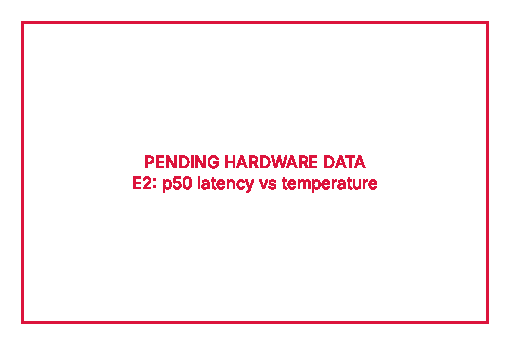
\includegraphics[width=\columnwidth]{figures/f_sustained.pdf}
\caption{Median latency of the nominal rung over a sustained run as CPU
temperature rises (E2).}\label{fig:sustained}
\end{figure}
\TBD{Describe the onset temperature and magnitude of latency drift and the
time to first firmware throttle.}

\subsection{Static versus adaptive (E3)}
\begin{table*}[t]
\centering\small
\caption{Static versus adaptive operation under sustained load (E3).}\label{tab:adaptive}
\begin{tabular}{lrrrrrrr}
\toprule
Arm & Runs & Mean FPS & p5 FPS & Throttled \% & $>$70\,\textdegree C \% & Max T & Switches/h \\
\midrule
Static nominal & \TBD{} & \TBD{} & \TBD{} & \TBD{} & \TBD{} & \TBD{} & \TBD{} \\
Static emergency & \TBD{} & \TBD{} & \TBD{} & \TBD{} & \TBD{} & \TBD{} & \TBD{} \\
SHADE & \TBD{} & \TBD{} & \TBD{} & \TBD{} & \TBD{} & \TBD{} & \TBD{} \\
SHADE + gate/shift & \TBD{} & \TBD{} & \TBD{} & \TBD{} & \TBD{} & \TBD{} & \TBD{} \\
SHADE + forecast & \TBD{} & \TBD{} & \TBD{} & \TBD{} & \TBD{} & \TBD{} & \TBD{} \\
\bottomrule
\end{tabular}
\par\smallskip\footnotesize Mean $\pm$ s.d. over runs; ambient, enclosure and cooling in Sec.~\ref{sec:setup}.
\end{table*}

\begin{figure}[t]\centering
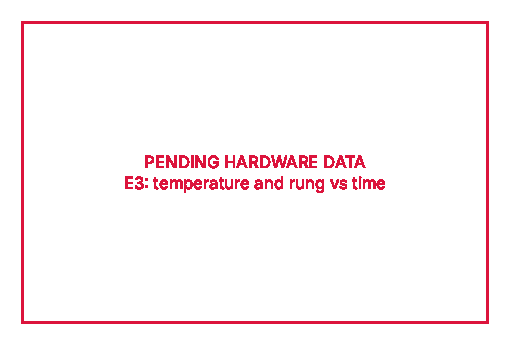
\includegraphics[width=\columnwidth]{figures/f_traces.pdf}
\caption{Temperature over time, static nominal versus \shade{} (E3, run 1).}\label{fig:traces}
\end{figure}
Relative to the static nominal arm, \shade{} changed throttled time from
\resStaticThrottled\% to \resShadeThrottled\%, the 5th-percentile frame rate from
\resStaticPfive{} to \resShadePfive{}~FPS and the mean frame rate from
\resStaticFps{} to \resShadeFps{}~FPS. \TBD{State plainly whether adaptation
paid: if mean throughput fell, say by how much and what it bought.}

\subsection{Swap cost (E4)}
\begin{table}[t]
\centering\small
\caption{Model-swap cost from the audit log (E4).}\label{tab:swap}
\begin{tabular}{lrrr}
\toprule
Quantity & n & Median & p95 \\
\midrule
Reference swap (ms) & \TBD{} & \TBD{} & \TBD{} \\
First-frame time (ms) & \TBD{} & \TBD{} & \TBD{} \\
Background load (s) & \TBD{} & \TBD{} & \TBD{} \\
\bottomrule
\end{tabular}
\end{table}

\TBD{Report the longest inter-frame gap during a background preload on the Pi and the
effect of the preload thread's niceness; our earlier 2-core x86 measurement showed
a preload can stall the loop, so this must be measured on the target.}

\subsection{Gating and shifting on real footage (E8)}
\begin{table}[t]
\centering\small
\caption{Gating and box shifting on real footage (E8, IoU 0.75).}\label{tab:gating-real}
\begin{tabular}{lrrrr}
\toprule
Arm & N & Calls & F1 & F1 (fast motion) \\
\midrule
hold & 4 & \TBD{} & \TBD{} & \TBD{} \\
hold & 8 & \TBD{} & \TBD{} & \TBD{} \\
shift & 4 & \TBD{} & \TBD{} & \TBD{} \\
shift & 8 & \TBD{} & \TBD{} & \TBD{} \\
gate & 4 & \TBD{} & \TBD{} & \TBD{} \\
gate & 8 & \TBD{} & \TBD{} & \TBD{} \\
gate+shift & 4 & \TBD{} & \TBD{} & \TBD{} \\
gate+shift & 8 & \TBD{} & \TBD{} & \TBD{} \\
\bottomrule
\end{tabular}
\par\smallskip\footnotesize Reference: detector on every frame of the same clips.
\end{table}

Gating removed \resGateSaving\% of detector calls at $N{=}4$ and shifting changed
F1 (IoU~0.75, fast motion, $N{=}8$) from \resShiftGain. \TBD{Break down by
clip type and report failures, e.g. small objects entering static scenes.}
For reference, the offline synthetic-pan study is in Table~\ref{tab:gating-synth}
and Fig.~\ref{fig:gating}.
\begin{table}[t]
\centering\small
\caption{Gating and shifting, real YOLOv8n on a synthetic pan of one image (offline, IoU 0.75).}\label{tab:gating-synth}
\begin{tabular}{lrrrr}
\toprule
Arm & N & Calls & F1 & F1 (fast pan) \\
\midrule
hold & 4 & 0.25 & 0.933 & 0.808 \\
shift & 4 & 0.25 & 0.958 & 0.889 \\
gate & 4 & 0.19 & 0.933 & 0.808 \\
gate+shift & 4 & 0.19 & 0.958 & 0.889 \\
hold & 8 & 0.12 & 0.873 & 0.639 \\
shift & 8 & 0.12 & 0.931 & 0.811 \\
gate & 8 & 0.09 & 0.874 & 0.639 \\
gate+shift & 8 & 0.09 & 0.928 & 0.811 \\
\bottomrule
\end{tabular}
\end{table}

\begin{figure}[t]\centering
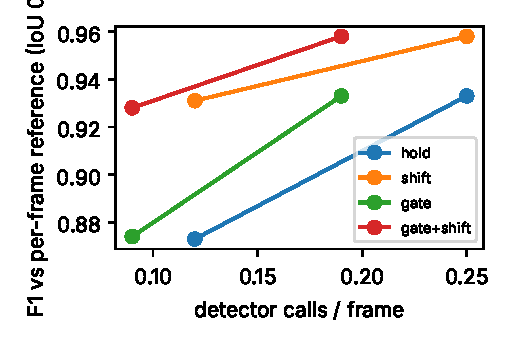
\includegraphics[width=\columnwidth]{figures/f_gating.pdf}
\caption{Agreement with per-frame detection versus detector calls (synthetic
pan, real YOLOv8n, IoU 0.75).}\label{fig:gating}
\end{figure}
